\documentclass[
    parskip=half, 
    twoside=false,
    twocolumn=true,
    fontsize=11pt,
]{scrarticle}
\usepackage{xcolor}
\definecolor{seeblau}{HTML}{00A9E0}
\definecolor{seegrau}{HTML}{9AA0A7}

\definecolor{seeblau1}{HTML}{CCEEF9}
\definecolor{seeblau2}{HTML}{A6E1F4}
\definecolor{seeblau3}{HTML}{59C7EB}
\definecolor{seeblau4}{HTML}{00A9E0}
\definecolor{seeblau5}{HTML}{008ECE}


\usepackage{graphicx}
\usepackage{amsmath}
\usepackage{subcaption}
\usepackage{wrapfig}
\usepackage[english]{babel}
\usepackage{blindtext}
\usepackage{microtype}
\usepackage{siunitx}
\usepackage[utf8]{inputenc}
\usepackage{csquotes}
\usepackage{nicefrac}
\usepackage[T1]{fontenc}
\usepackage{amsfonts}
\usepackage{amssymb}
\usepackage{tikz}

\usepackage{siunitx}

\usepackage{libertinus, libertinust1math}
\usepackage{roboto}

\setkomafont{disposition}{\normalfont\sffamily}


% not recommended with KOMA-script
% make table of contents sans-serif
% \usepackage{tocloft}
% \renewcommand\cftchappagefont{\normalfont}
% \renewcommand\cftchapfont{\normalfont}
% \renewcommand\cftchappresnum{\bfseries}
% \renewcommand\cftchapaftersnum{}
% \renewcommand{\cftchapfont}{\sffamily}
% \renewcommand{\cftsecfont}{\sffamily}
% \renewcommand{\cftsubsecfont}{\sffamily}
% \renewcommand{\cftchappagefont}{\sffamily}
% \renewcommand{\cftsecpagefont}{\sffamily}
% \renewcommand{\cftsubsecpagefont}{\sffamily}

% caption
\usepackage{caption}
\captionsetup{
	% font={sf},
	labelfont={sf, bf, color=seeblau},
	labelsep=quad,
	labelformat=simple,
}

% links
\usepackage{hyperref}
\hypersetup{
	colorlinks=true,
	linkcolor=seeblau,
	citecolor=seeblau,
	urlcolor=seeblau,
	% hidelinks=true
}

% bibliography
\usepackage[
	style=numeric-comp, % comp = compressed 4,5,6,7 -> 4-7
	sorting=none,		% Sort by appearance
	% autocite = superscript,
	% backref=true,
	hyperref=true,
	url=true,
	maxbibnames=100
]{biblatex}
\DefineBibliographyStrings{english}{%
    backrefpage  = {see p.}, % for single page number
    backrefpages = {see pp.} % for multiple page numbers
}

% remove issue
\AtEveryBibitem{%
  \clearfield{number}
}

\usepackage{float}
% \floatplacement{figure}{h}
% \floatplacement{table}{H}

% loosen float placement rules
\renewcommand{\topfraction}{0.8}
\renewcommand{\bottomfraction}{.8}
\renewcommand{\textfraction}{0.1}
\renewcommand{\floatpagefraction}{.9}
% make floats less likely to be placed on a separate page
\setcounter{totalnumber}{9}
\setcounter{topnumber}{9}
\setcounter{bottomnumber}{9}

% decrease space between floats and text
\setlength{\textfloatsep}{0.5cm}
\setlength{\floatsep}{0.5cm}


\usepackage{adjustbox}

\usepackage{datetime}
\newdateformat{dotdate}{
	\twodigit{\THEDAY}.\twodigit{\THEMONTH}.\THEYEAR
}
\newdateformat{monthyeardate}{%
  \monthname[\THEMONTH] \THEYEAR}


% header and footer
\usepackage[
  markcase=noupper
]{scrlayer-scrpage}% activates pagestyle scrheadings automatically
\clearpairofpagestyles
\setkomafont{pageheadfoot}{\normalfont\sffamily}
\setkomafont{pagenumber}{\normalfont\sffamily}
% \chead*{\color{seegrau} Draft \dotdate\today}
\ofoot*{\pagemark}
\ohead*{\rightmark}


\usepackage{ifthen}
\newcommand{\markieren}[4]{
    \ifthenelse{\equal{#1}{}}{}{\adjustbox{padding=3pt, bgcolor=seeblau1, margin=-1pt}{\strut{\sffamily\robotoMedium{#1}}}\\}
    \ifthenelse{\equal{#2}{}}{}{\adjustbox{padding=3pt, bgcolor=seeblau2, margin=-1pt}{\strut{\sffamily\robotoMedium{#2}}}\\}
	\ifthenelse{\equal{#3}{}}{}{\adjustbox{padding=3pt, bgcolor=seeblau3, margin=-1pt}{\strut{\sffamily\robotoMedium{#3}}}\\}
	\ifthenelse{\equal{#4}{}}{}{\adjustbox{padding=3pt, bgcolor=seeblau4, margin=-1pt}{\strut{\sffamily\robotoMedium{#4}}}}
}

\addbibresource{literature.bib}
\usepackage{listings}

\lstset{
    language=Python,                 % Language
    basicstyle=\ttfamily\small,       % Code font style
    keywordstyle=\color{blue},        % Keywords in blue
    stringstyle=\color{red},          % Strings in red
    commentstyle=\color{gray},        % Comments in gray
    % numbers=left,                     % Line numbers on the left
    numberstyle=\tiny,                 % Small line numbers
    stepnumber=1,                      % Show every line number
    % breaklines=true,                   % Line breaking
    mathescape=true
}


\begin{document}

\title{title}
\subtitle{subtitle}
\author{Aurel Müller-Schoenau, Leon Oleschko}
\date{\dotdate\today}


% make a custom title page
\begin{titlepage}
    \sffamily
    \vspace*{3cm}
    {
        \fontsize{32}{32}
        \markieren{}{}{}{Motencarlo}
    }
    \vspace{.25cm}\\
    {
        \Large
        Aurel Müller-Schoenau, Leon Oleschko\\
        Supervised by Philipp Baumgärtel
        \vspace{.05cm}\\
        22.01.2025
        \vspace{.25cm}\\
        \normalsize
        Physikalisches Fortgeschrittenenpraktikum 2\\
        Universität Konstanz
    }
    \vfill
    {
        \normalfont\normalsize
        In this experiment, we used Monte Carlo simulations to study the stochastic motion of a particle in various potential landscapes. We confirmed the expected diffusive behavior for a free particle, verified the equilibrium distributions for confined particles in potential wells and the normally distributed density in a harmonic potential. Additionally, we analyzed barrier crossing times in a double-well potential, demonstrating agreement with the Arrhenius law. The results validate the effectiveness of Monte Carlo methods in simulating statistical physics systems.
    }
    \vfill
    \begin{flushright}
        Available at \url{www.github.com/leoole100/fp2}.
    \end{flushright}
\end{titlepage}

\section{Introduction}
In physics research we ususally try to rely on very simplified model systems. This lets us investigate dynamics deterministically under controlled conditions to analyse each and every relevant interplay. However, nature is complex and modeling real systems may lead to the question - How do you analyse systems so complex they have a (practically) indefinite amount of degrees of freedom?\\
Statistical physics deals with this issue by making assumptions based on the idea that nature approaches thermodynamic equilibrium. This simplifies the dynamics of a single particle because one may assume the interactions with the rest of the system can be reduced to random interactions following a certain distribution. Computer-based methods making use of random numbers as means for simulation are generally called \textit{Monte-Carlo-Methods}.\\
In this experiment, we simulate the one-dimensional trajectory of a particle inside different energy potential landscapes under the influence of random kicks. Our goal is to confirm the theoretical models derived in statistical mechanics.

\section{Methods}
\begin{lstlisting}[caption={Python function used for time evolution.},label={lst:step},captionpos=b]
from numpy import exp
from numpy.random import random, choice

def $x_{n+1}$($x_n$, $V$, $\Delta x$=0.01):
  $\Delta x_n$ = choice([-1,1],len($x$))*$\Delta x$
  return $x$ + $\Delta x_n$*(
    random(len($x$)) < exp($-V(x+\Delta x_n)+V(x)$)
  )
\end{lstlisting}
To simulate the trajectory $x_t$ in a potential $V(x)$ the python function in \autoref{lst:step} is used.
This implements the \textit{Metropolis–Hastings Algorithm} \cite{noauthor_metropolis-algorithmus_2024}.
The position $x$ is updated at each timestep.
A candidate with $\Delta x_n \in \{\pm \Delta x\}$ is randomly chosen and accepted with the probability
$$ p(x_n \rightarrow x_{n+1}) = \text{min}\left[1,e^{-\frac{V(x_{n+1})-V(x_n)}{k_B T}}\right] \text{.}$$
$k_B T = 1$ is chosen to set the energy scale of the simulation.

To speedup the simulation of large ensembles a vector of multiple particle positions can be used for $x$.
The full code is available under \url{https://github.com/leoole100/fp2}.

\section{Results}
\subsection{Free Particle}
\begin{figure}
    \centering
    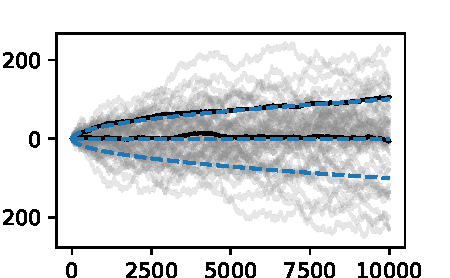
\includegraphics{figures/01 time trace.pdf}
    \caption{
        Time evolution of a free particle.
        Multiple time traces $x_n$ in gray, Assemble averages $\langle x_n\rangle, \sigma_n$ in black, expected averages in dashed blue.
    }
    \label{fig:pt1_trajectory}
\end{figure}

% TODO: Diagramme: Trajektorien, Mean Trajectorien, MSQ mit theoretischer Kurve

In the first part of this experiment, the simple goal was to get a simulation running with nothing more than a freely moving particle in one dimension. 
The potential is chosen to be $V(x)=0$ and the particles are initialized at $x_0=0$.
This results in Brownian Motion shown in \autoref{fig:pt1_trajectory}. Simulation data was generated for \SI{50} individual trajectories, each one being simulated for a total of $N=\SI{100000}{}$ timesteps. The expected result are freely diffusive dynamics, as shown in the plot.
The expected ensemble mean is $\langle x_n\rangle = 0$ and the standard deviation is $\sigma_n = \sqrt{\langle x_n^2 \rangle} = \sqrt{n}$ \autocite{noauthor_wiener_2025}.
This is also shown in the \autoref{fig:pt1_trajectory}.

\begin{figure}
    \centering
    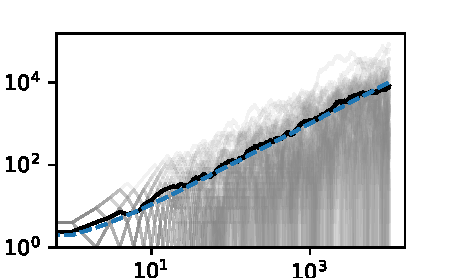
\includegraphics{figures/01 msd.pdf}
    \caption{
        Mean Square Displacement of a ensemble of 50 trajectories.
        Multiple time traces $x_n^2$ in gray, Assemble average in black, expected traces in dashed blue.
    }
    \label{fig:pt1_msd}
\end{figure}
Another way to describe the statistics of this process is the \textit{Mean Square Displacement} defined by $\langle x_n^2 \rangle$.
Since the displacements for different timesteps $n$ are uncorrelated, we expect that
\begin{align*}
    \langle x_n^2 \rangle 
    &= \left(\sum_{i=1}^n \Delta x_i\right)^2 \\
    &= 2 \cdot \underbrace{\sum_{i<j\leq n} \Delta x_i \Delta x_j}_{=0} + \sum_{i=1}^n \Delta x_i^2 \\ 
    &= n \cdot \Delta x^2
\end{align*}
The Mean Square Displacement averaged over all \SI{50}{} trajectories is shown in \autoref{fig:pt1_msd} alongside the matching theoretical prediction.


\subsection{Potential Well}
\begin{figure}
    \centering
    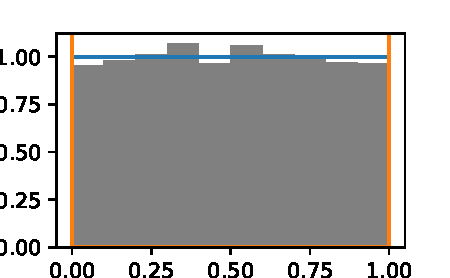
\includegraphics{figures/02 histogram.pdf}
    \caption{
        Histogram and potential over position of a particle in a potential well.
        Probability density $P(x)$ in units of $1/l$ in gray, expected probability density in blue, Potential $V(x)$ in orange
    }
    \label{fig:pt2_histogram}
\end{figure}
\begin{figure}
    \centering
    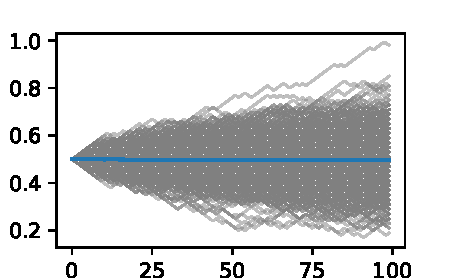
\includegraphics{figures/02 time evolution.pdf}
    \caption{
        Time evolution of a particle in potential well.
        Multiple time traces $x_n$ in gray, Assemble average of $\langle x_n\rangle$ in black, expected mean trace in dashed blue.
    }
    \label{fig:pt2_trajectory}
\end{figure}

Next we looked at a particle trapped inside a potential well with infinitely high walls.
This can be modelled with the potential
$$
V(x) = \begin{cases}
    0, &\text{if } 0\leq x\leq l\\
    \infty, &\text{otherwise}
\end{cases}
$$
where $l=1=100\;\Delta x$ is a characteristic length scale.
The potential is shown in \autoref{fig:pt2_histogram}.

The particles are initialized at $0.5 l$ and the time evolution is shown in \autoref{fig:pt2_trajectory}.
As one would expect, the trajectories begin like the the free timeevolution until it is confined by the wall.

The histogram in \autoref{fig:pt2_histogram} shows the average spacial distribution of all trajectories for a long evaluation time of \SI{100000}{} steps. 
It is flat, meaning that on average, the particle is able to visit each position of the potential with equal probability.
This confirms the expectation.
As the particle moves on the same grid $\{0, \Delta x, \cdots 1\}$ as is used for the histogram, the dip in the bin $0.48000000000000004$ to $0.49$ is presumably due to some numerical artefact.

The distribution from a random starting point is equal to waiting for the particles to randomly distribute in the well and taking the timeevolution after that.
But as this happens in a finite time, the histogram is the same as the one in the long time limit.

\subsection{Harmonic Potential}
\begin{figure}
    \centering
    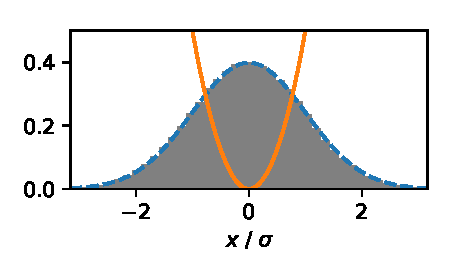
\includegraphics{figures/03 histogram.pdf}
    \caption{
        Histogram and potential over position of a particle in a harmonic potential.
        Probability density $P(x)$ in units of $1/\sigma$ in gray, expected probability density in blue, Potential $V(x)$ in units of $k_B T$ in orange
    }
    \label{fig:pt3_histogram}
\end{figure}

The harmonic potential appears in many real world cases, and any analytic potential can at least be approximated (locally) quadratically. In our case, the idea is to simulate a particle trapped inside optical tweezers, the resulting potential is nearly harmonic as we learned from one of our previous experiments:
$$ V(x) = \frac{1}{2 \sigma^2} x^2$$
where $\sigma = 1000 \Delta x$ is a characteristic length scale.
This potential is shown in \autoref{fig:pt3_histogram}.
\\
Unlike in the previous sections, the particle can now explore areas but only if it gains enough energy. The resulting spacial distribution is
$$
\label{eq:canonical_dist}
 P(x) \propto e^{-\frac{V(x)}{k_B T}} = e^{-\frac{x^2}{2 \sigma^2}}.
$$

Our simulation was run for \SI{100000}{} timesteps and we simulated $50$ trajectories. 
The results are shown in \autoref{fig:pt3_histogram} in the form of a histogram.
The spacial distribution follows a normal Distribution as expected.


\begin{figure}
    \centering
    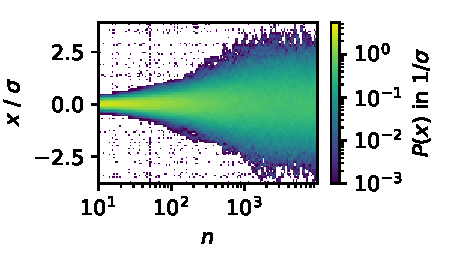
\includegraphics{figures/03 histogram evolution.pdf}
    \caption{
        Evolution of the probability density for the particles in a harmonic potential.
    }
    \label{fig:pt3_histogram_time}
\end{figure}
To see how the distribution evolves over time from the starting condition of $x_0=0$ to the derived normal distribution, it is shown over time in \autoref{fig:pt3_histogram_time}.
The distribution stays normally distributed with a increasing standard deviation, until the derived limit of $\sigma$ is reached.

\subsection{Double Well}
\begin{figure}
    \centering
    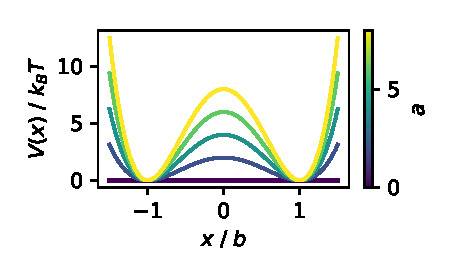
\includegraphics{figures/04 potential.pdf}
    \caption{Double well potential for different $a$.}
    \label{fig:pt4_potential}
\end{figure}
In the final part of the experiment we simulated a particle trapped inside a double-well potential given by
$$V(x) = a\left(\left(\frac{x}{b}\right)^2-1\right)^2$$
which is a fourth order polynomial with minima at $x=\pm b$ and a local maximum inbetween at $V(x=0)=a$.
As the $b$ only scales $x$ relative to $\Delta x$, this can be taken out into the length scale.
Such a rescaling is not done with $a$ on the energy, as it changes the dynamics non trivially.
The potential is shown in \autoref{fig:pt4_potential} for different $a$.
Letting the particle evolve, it delves inside one of the potential wells first, until after some time it manages to climb and surpass the barrier imposed by the local maximum at $x=0$. 
Our goal was to find out how the time it takes on average $\langle n \rangle$ to complete one such jump depends on the height of the barrier $a$.

\begin{figure}
    \centering
    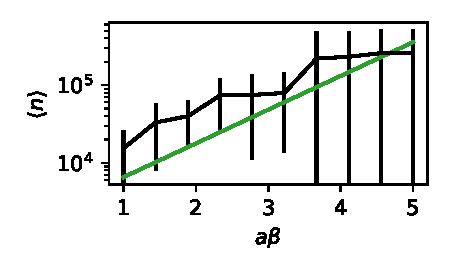
\includegraphics{figures/04 chem.pdf}
    \caption{
        Mean time to jump from $x=b$ to $x=0$ for different $a$ in the double well potential.
        With a exponential fit of $\langle n \rangle = 2400\pm 340 \exp\left(a\right)$.
    }
    \label{fig:pt4_arrhenius}
\end{figure}
To do this, we simulated many trajectories for different values of $a$. The resulting mean jump times -- that is the time between initialisation and the point where the particle reaches the maximum of the barrier -- are plotted over the parameter $a$ in \autoref{fig:pt4_arrhenius}. They increase exponentially with $a$ according to $\langle n \rangle = (2400\pm 340) \exp\left(a\right)$ like expected due to the \textit{Arrhenius law} \autocite{noauthor_arrhenius_2024}.
Where the Escape Rate $2400\pm 340$ is in the units of the time between the steps.

\pagebreak
\section{Conclusion}
The \textit{Monte Carlo Simulation} experiment is a small introduction into physical simulation of systems described by statistical physics. We demonstrated how such simulations are set up for different scenarios.\\
In the first part of the experiment, we simulated a freely moving particle and were able to confirm the viability of the law of free diffusion. 
When constraining the particle inside a potential well, we found the expected flat spacial distribution after sufficiently long simulation time -- this is in line with the canonical distribution introduced in the following chapter, which states that the probability of a particle residing at some position should only depend on the potential energy at that position.
The spacial distribution we computed for the harmonic potential using the Metropolis algorithm resembles the expected Gaussian distribution.\\
In the final part we tried to find out how the average time to cross a potential barrier depends on the barrier height to obtain the Arrhenius law. 

\addcontentsline{toc}{section}{Literature}
\nocite{*}
\printbibliography

\end{document}
